\documentclass[11pt,english]{article}
\usepackage[T1]{fontenc}
\usepackage[utf8]{inputenc}
\usepackage[english]{babel}
\usepackage[pdfauthor={Lars Maiwald, Kevin Siebert}]{hyperref}
\usepackage{amsthm}
\usepackage{amssymb}
\usepackage{amsmath}
\usepackage{mathtools}
\usepackage{comment}
\usepackage{pdfpages}
\usepackage{fancyhdr}
\usepackage[headheight=14pt]{geometry}
\usepackage{graphicx}
\usepackage{caption}
\usepackage{subcaption}
\usepackage{siunitx}
\usepackage{csquotes}
\usepackage{hyphenat}
\usepackage{float}
\usepackage{xcolor}
\usepackage{cleveref}
\usepackage{listings}
\usepackage[lighttt]{lmodern}
\usepackage{appendix}
\usepackage{booktabs}
\usepackage[affil-it]{authblk}
\usepackage[backend=biber,style=phys,biblabel=brackets,pageranges=false,sorting=nyt]{biblatex}
\usepackage{multicol}
\usepackage{watermark}
%\addbibresource{}

\lstdefinestyle{CppStyle}{
  language=C++,
  stepnumber=1,
  numbersep=10pt,
  tabsize=4,
  showspaces=false,
  showstringspaces=false
}
\lstdefinestyle{PseudoStyle}{
  basicstyle=\small\ttfamily,
  stepnumber=1,
  numbersep=10pt,
  tabsize=4,
  showspaces=false,
  showstringspaces=false,
  keywordstyle=\color{black}\bfseries\em,
  keywords={,input, output, return, datatype, function, in, if, else, foreach, while, begin, end, }
}
\lstset{basicstyle=\small\ttfamily, style=CppStyle}

\crefname{equation}{}{}
\Crefname{equation}{\text{Equation}}{\text{Equations}}
% \crefname{section}{\text{Kapitel}}{\text{Kapitel}}
% \Crefname{section}{\text{Kapitel}}{\text{Kapitel}}
% \crefname{table}{\text{Tab.}}{\text{Tab.}}
% \Crefname{table}{\text{Tabelle}}{\text{Tabellen}}
% \crefname{figure}{\text{Abb.}}{\text{Abb.}}
% \Crefname{figure}{\text{Abbildung}}{\text{Abbildungen}}

\numberwithin{equation}{section}

%\hyphenation{Mathe-matik wieder-gewinnen}

\sisetup{
locale = DE,
range-phrase = \ldots,
separate-uncertainty=true,
scientific-notation=true,
}

\geometry{
  a4paper,
  left=2.5cm,
  right=2.5cm,
  top=3cm,
  bottom=3cm
}

\renewcommand{\footrulewidth}{0.4pt}
\renewcommand{\headrulewidth}{0.4pt}
\pagestyle{fancy}
\fancyhf{}
\rhead{Maiwald, Siebert}
%\lfoot{}
\lhead{\slshape\nouppercase{\leftmark}}
\cfoot{\thepage}
%\pagestyle{empty}

\hypersetup{
    colorlinks=true,
    linkcolor=blue,
    filecolor=magenta,      
    urlcolor=magenta,
    citecolor=green,
}
\urlstyle{same}

\graphicspath{ {resources/figures/} }

\allowdisplaybreaks

% \setlength\parindent{0pt}

%Einige nützliche Definitionen
\newcommand{\deriv}[2]{\frac{\mathrm{d} #1}{\mathrm{d} #2}}
\newcommand{\pderiv}[2]{\frac{\partial #1}{\partial #2}}
% \newcommand{\kommut}[2]{\left[ #1, #2 \right]}
% \newcommand{\tagthis}[1]{\addtocounter{equation}{1}\tag{\theequation}\label{#1}}
% \newcommand{\tagit}{\addtocounter{equation}{1}\tag{\theequation}}
% \DeclarePairedDelimiter\bra{\langle}{\rvert}
% \DeclarePairedDelimiter\ket{\lvert}{\rangle}
% \DeclarePairedDelimiterX\braket[2]{\langle}{\rangle}{#1 \delimsize\vert #2}
% \DeclarePairedDelimiterX\expval[2]{\langle}{\rangle}{#2 \delimsize\vert #1 \delimsize\vert#2}
% \DeclarePairedDelimiterX\matrixel[3]{\langle}{\rangle}{#1 \delimsize\vert #2 \delimsize\vert#3}
% \DeclarePairedDelimiterX\expv[1]{\langle}{\rangle}{#1}

\newcommand{\ie}{\textit{i.e.} }
\newcommand{\eg}{\textit{e.g.} }

\lstset{
	escapeinside={/*@}{@*/}, language=C++,
	basicstyle=\fontsize{8.5}{12}\selectfont,
	numbers=left,numbersep=2pt,xleftmargin=2pt,frame=tb,
    columns=fullflexible,showstringspaces=false,tabsize=4,
    keepspaces=true,showtabs=false,showspaces=false,
    backgroundcolor=\color{white}, morekeywords={inline,public,
    class,private,protected,struct},captionpos=t,lineskip=-0.4em,
	aboveskip=10pt, extendedchars=true, breaklines=true,
	prebreak = \raisebox{0ex}[0ex][0ex]{\ensuremath{\hookleftarrow}},
	keywordstyle=\color[rgb]{0,0,1},
	commentstyle=\color[rgb]{0.133,0.545,0.133},
	stringstyle=\color[rgb]{0.627,0.126,0.941}
}

\graphicspath{{./resources/images/}}

\thiswatermark{\centering \put(326.5,-68.0){\includegraphics[scale=1.2]{sciences_en.png}}}

\usepackage{abstract}
\newcommand{\myabstract}[1]{
\twocolumn[
  \maketitle             % full width title
  \begin{onecolabstract} % ditto abstract
    {#1}
  \end{onecolabstract}
\vspace{\baselineskip}
]}
\usepackage[backend=biber, style=phys]{biblatex}
\addbibresource{resources/references.bib}

\title{\textbf{Report: \\ Deep learning final project (miniprojects)}}
\author{Kevin Siebert%
	\thanks{\textsc{}s{\href{mailto:Kevin.Siebert@etu.unige.ch}{Kevin.Siebert@etu.unige.ch}}}}
\affil{Department of Informatics, Faculty of Science, \\ University of Geneva}
\date{Dated: \today}

\begin{document}
	\maketitle
	\vspace{-20pt}
	\begin{abstract}
		This is a report on the solution of the two mini projects proposed as a final project for the course Deep Learning (14X050). The solutions consists of this report and a GitHub archive containing the corresponding code (\thanks{\href{https://github.com/I-am-Rudi/DL_FinalProject}{Github Archive}}).
	\end{abstract}
	
	\section{Project} \label{sec:Proj1}
	\vspace{-10pt}
	\subsection{Introduction}
	The main goal of the first project is to compare the performance of basic neural network architectures. This is done with respect to a specific classification task where the network is supposed to predict the relationship (smaller or equal / larger) between two numbers of the MNIST dataset. A small selection from this dataset can be seen in \cref{fig:ex_pair}.
	
	\begin{figure}[H]
		\centering
		\includegraphics[width = .30\textwidth]{pair_example.png}
		\caption{Small selection of inputs from the dataset where every row represents on input and the caption show the corresponding target classes.}
		\label{fig:ex_pair}
	\end{figure} 


	\subsection{Architectures} \label{ssec:Architectures}
	For the structure of the networks, four variable architectures where chosen. For all architectures there is one one version which starts with several convolutional and Batchnorm layers and is followed by linear layers, another which is fully convolutional and every architecture has the possibility to switch between several or one output neuron depending on whether one-hot encoded labels are used. 
	
	The fully convolutional networks are created on the basis of the mixed networks at initialization through the function \lstinline|convolutionize| which is based on the \lstinline|convolutionize| function \cite{Fleuret2022} defined in the lectures. They are not transformed after training but at initialization so they are trained as fully convolutional networks. From this point on not calling  \lstinline|convolutionize| will be the norm for project one. Whenever fully covolutional networks are used it will be explicitly specified.
	
	One-hot encoding is specified through the variable \lstinline|one_hot_encoding| at initialization and is enabled for all additional functions by the same variable. From this point on one-hot encoding will be the norm for project one. Whenever one-hot encoding is turned of it will be explicitly specified.
	
	All architectures use ReLU as their internal activation functions and Sigmoid as their output activation. All models are initialized with 64, 64 and 32 for the number of neurons in the main branch for the hidden Linear layers.
	
	The first implemented architecture can be seen in \cref{fig:sn} it represents the ``naive'' approach where the images are passed through separate convolutional layers to extract their feature. The results are concatenated flattened and passed through fully connected linear layers/convolutional layers for the actual classification. This architecture will be called ``simple network'' (SN) from now on.
	
	\begin{figure}[H]
		\centering
		\includegraphics[width = .75\textwidth]{Simple_network.png}
		\caption{Diagrammatic visualization of the architecture for the simple network. (figure made using Inkscape)}
		\label{fig:sn}
	\end{figure}

	Of course an architecture like \cref{fig:sn} wastes some learning potential by separating the feature extraction. Therefore an attempt on improvement is made through the architecture in \cref{fig:ws} from now on called ``weight sharing network'' (WSN). Here, we do the feature extraction by passing Number 1 as well as Number 2 (one after the other) threw the first two convolutional layers, then concatenate and continue.
	
	\begin{figure}[H]
		\centering
		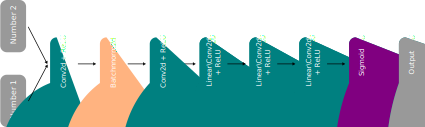
\includegraphics[width = .75\textwidth]{Weight_sharing_network.png}
		\caption{Diagrammatic visualization of the architecture for the weight sharing network.(figure made using Inkscape)}
		\label{fig:ws}
	\end{figure}

	The following two architectures rely on the concept of auxiliary classifiers as described in \cite{Szegedy2014}. The basic idea is to branch of the main architecture at some point to do the same or another classification task from the input. This part is also trained and the loss is added (usually multiplied by a some fraction smaller than one) to the loss of the main branch. This part is usually discarded when evaluating the model.
	
	\Cref{fig:saux} takes the most simple approach to this concept by branching of and trying to perform the same classification as the main branch and will therefore be called ``Simple auxiliary classifier model'' (SAUX) from now on.
	
	\begin{figure}[H]
		\centering
		\includegraphics[width = .75\textwidth]{Simple_aux_network.png}
		\caption{Diagrammatic visualization of the architecture for the simple auxiliary neural network.(figure made using Inkscape)}
		\label{fig:saux}
	\end{figure}
	
	Another approach could be to use the information about the classes of the respective numbers from the MNIST. \Cref{fig:caux} introduces this concept by having an auxiliary classifier branch just after the initial feature extraction to find the classes of the respective numbers. This architecture will be called ``auxiliary classifier using classes'' (CAUX) from now on.
	
	\begin{figure}[H]
		\centering
		\includegraphics[width = .75\textwidth]{Classes_aux_network.png}
		\caption{Diagrammatic visualization of the architecture for the auxiliary neural network using the numbers classes. (figure made using Inkscape)}
		\label{fig:caux}
	\end{figure}

	For both auxiliary architectures the modification specified at the start of this section are also imposed on the auxiliary classifiers. Both architectures keep the structure of the WSN for the initial feature extraction.
	
	\subsection{Training}
	
	All the Architectures were trained for 100 epochs, which was repeated for 150 times while logging the test accuracy to calculate the mean values and standard deviation for the results of that experiment. The actual Training and testing is performed by the \lstinline|Teacher| class which stores the train and test data and whose methods are the actual train and test function of the model. The whole process for the analysis is performed by the \lstinline|run_analysis| function which returns the name of the model input, the mean and the standard deviation for use in further analysis or visualization. All models with one-hot encoding where trained using the \lstinline|CrossEntropyLoss| optimizer and all the models without one-hot encoding where trained using the \lstinline|MSELoss| optimizer.
	
	All models where trained with a learning rate of \lstinline|0.01| and a batch size of \lstinline|50|. These parameters remained fixed for the whole analysis in project one to keep the results as comparable as possible.
  	
  	\subsection{Results} \label{ssec:Results1}
  	
  	As a starting point the different architectures are compared in their standard forms (one-hot encoding and not fully convolutional) as specified in \cref{ssec:Architectures}. The results of this comparison can be seen in \cref{fig:comp_normal-normal}. \Cref{fig:normal-normal:sn-ws} shows the WSN performing better on average than the SN. not only does it reach a higher value at the end of the training, it also as a steeper slope for the evolution of the test accuracy. This development is consistent with the ideas behind the WSN eplained in \cref{ssec:Architectures}. 
  	
  	The WSN is then compared to the SAUX with the result of them having nearly indistinguishable performance in the comparison \cref{fig:normal-normal:ws-saux}.
  	
  	\Cref{fig:normal-normal:saux-caux} shows the comparison between SAUX and CAUX, where SAUX seems to perform better overall with both architectures starting out very similar but the SAUX plateaus less agressivly. This result is unexpected as one might guess the introduction of additional informattion might have let to a boost in performance. 
  	
	\begin{figure*}
		\centering
		\begin{subfigure}[b]{0.475\textwidth}
			\centering
			\includegraphics[width=\textwidth]{compare/normal-normal/Comparison_Simple_convolutional_network_Weight_sharing_network.png}
			\caption[]%
			{{\small Simple network}}
			\label{fig:normal-normal:sn-ws}    
		\end{subfigure}
		\hfill
		\begin{subfigure}[b]{0.475\textwidth}  
			\centering 
			\includegraphics[width=\textwidth]{compare/normal-normal/Comparison_Weight_sharing_network_Simple_Auxiliary_classifier_network.png}
			\caption[]%
			{{\small Weight sharing network}}
			\label{fig:normal-normal:ws-saux} 
		\end{subfigure}
		\vskip\baselineskip
		\begin{subfigure}[b]{0.475\textwidth}   
			\centering 
			\includegraphics[width=\textwidth]{compare/normal-normal/Comparison_Simple_Auxiliary_classifier_network_Auxiliary_classifier_network_using_classes.png}
			\caption[]%
			{{\small Simple auxiliary classifier network}} 
			\label{fig:normal-normal:saux-caux}   
		\end{subfigure}
		\hfill
		\caption[]
		{The mean and standard deviation of the test accuracy compared over the course of 100 epochs calculated for 150 trials. For the architectures in their standard form.} 
		\label{fig:comp_normal-normal}
	\end{figure*}

	The next group of comparisons in \cref{fig:comp_conv-normal} shows the performance of the networks from \cref{fig:comp_normal-normal} against their fully convolutional equivalent. Sadly no significant improvement in performance is observable. A reason for that might be that the networks are not taking full advantage of the possibilities of the convolutional layers as they are mere translations of the mixed architectures.

	\begin{figure*}
		\centering
		\begin{subfigure}[b]{0.475\textwidth}
			\centering
			\includegraphics[width=\textwidth]{compare/fc-normal/Comparison_Simple_convolutional_network_Fully_convolutional_network.png}
			\caption[]%
			{{\small Simple network}}    
		\end{subfigure}
		\hfill
		\begin{subfigure}[b]{0.475\textwidth}  
			\centering 
			\includegraphics[width=\textwidth]{compare/fc-normal/Comparison_Weight_sharing_network_Fully_convolutional_weight_sharing_network.png}
			\caption[]%
			{{\small Weight sharing network}} 
		\end{subfigure}
		\vskip\baselineskip
		\begin{subfigure}[b]{0.475\textwidth}   
			\centering 
			\includegraphics[width=\textwidth]{compare/fc-normal/Comparison_Simple_Auxiliary_classifier_network_Fully_convolutional_auxiliary_classifier_network.png}
			\caption[]%
			{{\small Simple auxiliary classifier network}}    
		\end{subfigure}
		\hfill
		\begin{subfigure}[b]{0.475\textwidth}   
			\centering 
			\includegraphics[width=\textwidth]{compare/fc-normal/Comparison_Auxiliary_classifier_network_using_classes_Fully_convolutional_auxiliary_classifier_network_using_classes.png}
			\caption[]%
			{{\small Auxiliary classifier network (number classes)}}    
		\end{subfigure}
		\caption[]
		{The mean and standard deviation of the test accuracy compared over the course of 100 epochs calculated for 150 trials. For the architectures in their standard form.} 
		\label{fig:comp_conv-normal}
	\end{figure*}

	In contrast the switch to non-one-hot encoding visible in \cref{fig:comp_normal-oh} let to better performance of the SN, WSN, SAUX with the most significant improvement for the SN and barely significant for the WSN. The CAUX was unable to learn any significant structure from the dataset without one-hot encoding. This is probably due to the fact that while one output neuron might be well suited for a binary output having ten classes differentiated using one output neuron is more difficult. For the CAUX a mixed structure (main branch fully convolutional and auxiliary classifier unchanged) could be a better solution.
	
	\begin{figure*}
		\centering
		\begin{subfigure}[b]{0.475\textwidth}
			\centering
			\includegraphics[width=\textwidth]{compare/oh-normal/Comparison_Simple_convolutional_network_Simple_convolutional_network_one_hot_labels=False.png}
			\caption[]%
			{{\small Simple network}}    
		\end{subfigure}
		\hfill
		\begin{subfigure}[b]{0.475\textwidth}  
			\centering 
			\includegraphics[width=\textwidth]{compare/oh-normal/Comparison_Weight_sharing_network_Weight_sharing_network_one_hot_labels=False.png}
			\caption[]%
			{{\small Weight sharing network}} 
		\end{subfigure}
		\vskip\baselineskip
		\begin{subfigure}[b]{0.475\textwidth}   
			\centering 
			\includegraphics[width=\textwidth]{compare/oh-normal/Comparison_Simple_Auxiliary_classifier_network_Simple_Auxiliary_classifier_network_one_hot_labels=False.png}
			\caption[]%
			{{\small Simple auxiliary classifier network}}    
		\end{subfigure}
		\hfill
		\caption[]
		{The mean and standard deviation of the test accuracy compared over the course of 100 epochs calculated for 150 trials. For the architectures in their standard form.} 
		\label{fig:comp_normal-oh}
	\end{figure*}

	With the knowledge from \cref{fig:comp_conv-normal,fig:comp_normal-oh} only two comparisons are required to decide on the best performing network of this analysis. Namely the comparisons between the models without one-hot encoding as shown in \cref{fig:comp_int}. We can conclude that, by a small margin the SAUX without one-hot encoding delivered on average the best results for the architectures tested in this analysis.

	\begin{figure*}
		\centering
		\begin{subfigure}[b]{0.475\textwidth}
			\centering
			\includegraphics[width=\textwidth]{compare/interesting/Comparison_Simple_convolutional_network_one_hot_labels=False_Weight_sharing_network_one_hot_labels=False.png}
			\caption[]%
			{{\small Simple network}}    
		\end{subfigure}
		\hfill
		\begin{subfigure}[b]{0.475\textwidth}  
			\centering 
			\includegraphics[width=\textwidth]{compare/interesting/Comparison_Weight_sharing_network_one_hot_labels=False_Simple_Auxiliary_classifier_network_one_hot_labels=False.png}
			\caption[]%
			{{\small Weight sharing network}} 
		\end{subfigure}
		\hfill
		\caption[]
		{The mean and standard deviation of the test accuracy compared over the course of 100 epochs calculated for 150 trials. For the architectures in their standard form.} 
		\label{fig:comp_int}
	\end{figure*}

	\subsection{Conclusion}
	Four different base architectures and their modifications where tested during this project. In the case of one-hot encoding the best performing models are WSN and SAUX with nearly indistinguishable performance. In the case of non-one-hot encoding the best performing architecture found was SAUX. 
	
	In both cases CAUX performed worse than SAUX and WSN which is surprising but might be changed with a more sophisticated architecture for this type of classifier.
	
	No significant improvement was found using fully convolutional architectures but as explained in \cref{ssec:Results1} the networks as proposed in \cref{ssec:Architectures} do not take full advantage of the possibilities provided by the convolutional layers.

	\section{Project} \label{sec:Proj2}
	\vspace{-10pt}
	
	\subsection{Introduction} \label{ssec:Intro2}
	The goal of this project is to create a framework for constructing neural networks. Here, only the tensor functionalities of the PyTorch library should be used, especially not making use of the \lstinline|torch.nn| module and the autograd functions of Pytorch.
	
	There are five modules that are required to be implemented: Linear (fully connected layer), ReLU, Tanh, Sequential and LossMSE.
	
	To test the framework, a model with 2 input neurons at least three hidden layers of 25 neurons and 1 output neuron is created and trained on a test dataset. 
	
	The dataset used for testing is a standard choice in machine learning. Points are created uniformly over a subspace of $\mathbb{R}$ then all points inside a specified circle are classified as target 1 and outside the circle they are classified as target 0. For this project the circle is specified to have a radius of $\frac{1}{\sqrt{2 \pi}}$ centered at $x=0.5$ and $y=0.5$. The subspace is chosen to be $[0, 1]^2$. An example of the created dataset is visualized in \cref{fig:circleset}
	
	\begin{figure}
		\centering
		\includegraphics[width = .85\textwidth]{
			circleset.png}
		\caption{Test dataset for Project 2. Points inside a circle of radius $\frac{1}{\sqrt{2 \pi}}$ centered at $x=0.5$ and $y=0.5$ are classified as target 1 and outside the circle they are classified as target 0. Points are uniformly generated over $[0, 1]^2$.}
		\label{fig:circleset}
	\end{figure}  
	
	\subsection{The framework} \label{ssec:framework}
	
	\subsubsection{Base}
	
	As a Base Class 
	
	\begin{lstlisting}
		class Module:
		def __init__(self):
		self.has_params = False
		self.device = torch.device('cpu')
		
		# Defining __call__ method to keep the easy syntax for the forward prop
		def __call__(self, *input):
		return self.forward(*input)
		
		def forward(self, input):
		raise NotImplementedError
		
		def backward(self, gradwrtoutput):
		raise NotImplementedError
		
		def params(self):
		return []
	\end{lstlisting}
	
	was implemented as suggested in the task, the \lstinline|__call__| function was defined to be able to call the method \lstinline|forward| with \lstinline|Module()|.
	
	Building on that these base classes where made: 
	
	\begin{lstlisting}
		class Activation(Module):
		
		def __call__(self, input):
		self.x = self.forward(input)
		return self.x
		
		def backward(self, prev_layer, grad, loss = False):
		if loss:
		return torch.einsum("ik,jk->ij", prev_layer.derivative(self.x, activation=True), grad) 
		else:
		return torch.einsum("ik,jk->ji", prev_layer.derivative(self.x, activation=True), grad) 
		def to_device(self, device):
		self.device = device
	\end{lstlisting}
	
	\begin{lstlisting}
		class Optimizer(Module):
		def __init__(self, lr, batch_size, device=None):
		super().__init__()
		self.lr = torch.tensor([lr])
		self.has_params = True
		self.batch_size = torch.tensor([batch_size])
		
		def params(self):
		return [self.lr]
		
		def to_device(self, device):
		self.lr = self.lr.to(device)
		self.batch_size = self.batch_size.to(device)
		self.device = device
	\end{lstlisting}	
	
	\begin{lstlisting}
		class Loss(Module):
		def __init__(self, target):
		self.target = target  # I choose this initialization to make the loss compatible with the Backpropagation 
	\end{lstlisting} 
	
	\begin{lstlisting}
		class Model(Module):
		"""Base class for defining general models"""
		
		def __init__(self):
		super().__init__()
		self.has_params = True
		
		def save(self, filename, path=None):
		if path == None:
		with open(os.path.join(os.path.curdir, "saved_models", filename + ".pkl"), 'wb') as f:
		pickle.dump(self, f)
		else:
		try:
		with open( path + filename + ".pkl", 'wb') as f:
		pickle.dump(self, f)
		
		except:
		raise Exception("Please enter a valid path when using the optional path argument!")
	\end{lstlisting}
	
	They should allow too add new activations, losses, optimizers and more complex models than Sequential more quickly if needed. The model class provides a save function to store a model using the pickle library. The model can then be loaded into a variable using the \lstinline|load_model| function.
	
	All Modules posses a method \lstinline|to_device| which transfers all their parameters to the specified device and changes the parameter \lstinline|Module.device| to the specified device and therefore enabling CUDA support for the framework. All Modules posses a forward and a backward method except for \lstinline|Loss| and \lstinline|Optimizer|. All classes that can act as layers of a network and the loss are implemented with a method that returns their derivative.
	
	\subsubsection*{Forward pass}
	
	The forward pass for the modules is fairly straight forward as the definitions of the required functions are well known and can just be translated into code from the literature \cite{Fleuret2022,Goodfellow-et-al-2016}. With the only addition that the respective results are stored inside the class object for later use in the backward pass. Two forward methods might be worth mentioning. For the Tanh it is implemented using a second class for Sigmoid as they are closely related and then the Sigmoid function is implemented too without additional effort.
	
	\begin{lstlisting}
		class Sigmoid(Activation):
		
		def forward(self, input):
		return 1/(1+torch.exp(-input))
		
		def derivative(self, input, activation = False):
		if activation:
		raise Exception("Chaining of two activation functions directly after one another!")
		
		return self.forward(input) * (1 - self.forward(input))
		
		class Tanh(Activation):
		
		def __init__(self):
		super().__init__()
		self.sigmoid = Sigmoid()
		
		def forward(self, input):
		return 2 * self.sigmoid.forward(2 * input) - 1
		
		def derivative(self, input, activation = False):
		if activation:
		raise Exception("Chaining of two activation functions directly after one another!")
		
		return 4 * self.sigmoid.derivative(2*input)  # chain rule  
	\end{lstlisting}
	
	And the forward propagation of Sequential, which is just the chaining of 
	all the individual forward calls.
	
	\begin{lstlisting}
		def forward(self, input):
		for layer in self.layers:
		input = layer(input)
		
		return input
	\end{lstlisting}

	In contrast the backward propagation is way more nuanced. The general equations can be found in various resources like \cite{Fleuret2022,Goodfellow-et-al-2016}. For the case of the sequential model a more or less simple implementation is possible. Except for the first step of the backward propagation which includes the loss at every step corresponding to a layer the gradient (of at least one parameter) is calculated using only the derivative of the previous layer, the gradient of the previous layer and information and the forward pass result of the current layer (the direction being backwards in the graph). 
	
	Therefore we can make use of the already implemented derivative method and pass the previous layer as well as the gradient of its backward pass to the backward method of the current layer and use the information that has been stored during the forward pass. With one addition: When two Linear layers follow each other the previous one returns \lstinline|1| as its derivative, we can account for most possible architectures that can be created using \lstinline|Sequential|.
	
	Then for the linear layer the backward pass is implemented as:
	
	\begin{lstlisting}
		def backward(self, prev_layer, grad):
		self.db = prev_layer.derivative(self.s) * grad
		#self.db = torch.einsum("ik,jk->ij", prev_layer.derivative(self.s), grad)
		self.dw = torch.einsum('ik,ij->ikj', self.db, self.x)
		return self.db
	\end{lstlisting} 
	
	The activation backward pass is implemented as:
	
	\begin{lstlisting}
		def backward(self, prev_layer, grad, loss = False):
		if loss:
		return torch.einsum("ik,jk->ij", prev_layer.derivative(self.x, activation=True), grad) 
		else:
		return torch.einsum("ik,jk->ji", prev_layer.derivative(self.x, activation=True), grad) 
	\end{lstlisting}

	To get the backward pass for the whole Sequential model we use these methods in the \lstinline|Sequential.backward| method:
	
	\begin{lstlisting}
		def backward(self, loss):  # the loss functions will be initialized with target, they get one parameter as an instance which will be the output
		
		grads = [torch.tensor([1]).unsqueeze(1).to(self.device)]  # makes the Backprop of the loss work even if the ouput layers is not an activation
		self.layers.append(loss)
		self.layers = self.layers[::-1]
		
		for i in range(1, len(self.layers)):
		if i == 1:
		grads.append(self.layers[i].backward(self.layers[i-1], grads[i-1], loss = True))
		else:
		grads.append(self.layers[i].backward(self.layers[i-1], grads[i-1]))
		
		
		self.layers = self.layers[::-1]
		self.layers = self.layers[:-1]  # reformat the layer variable
		grads = grads[1:]
		grads = grads[::-1]
		return grads
	\end{lstlisting}
	
	After the gradient is calculated the models parameters need to be updated. As \lstinline|Linear| is the only layer with parameters in this example, the \lstinline|update_params| function is implemented for this module:
	
	\begin{lstlisting}
		def update_params(self, optimizer):
		if self.bias:
		self.b -= optimizer(self.db)
		self.w -= optimizer(self.dw)
	\end{lstlisting}
	
	The model \lstinline|Sequential| has a method \lstinline|update_params| which calls the \lstinline|update_params| of all layers with parameters (i.e. only linear layers in this case).
	
	Which concludes the basic tools needed to build a simple sequential neural network.
	
	\section{Training} \label{ssec:Training}
	
	Inside of every training function there is the sequence of calculating the output and doing backward pass and updates. In this framework as specified in \cref{ssec:framework} this sequence is:
	
	\begin{lstlisting}
		output = model(inputs)
		
		optim = nn.SGD(lr, inputs.shape[0])
		optim.to_device(self.device)
		
		loss = nn.MSE(targets)
		
		grads = model.backward(loss)
		model.update(optim)
	\end{lstlisting} 
	
	The framework was set up in a way such that whenever parameters inside the model are changed during training, this is done by a method of the model itself to stay in line with the usual conventions of object oriented programming. As opposed to \lstinline|torch.nn| where the backward pass is performed by the loss function object and the update is performed by the optimizer object.
	
	The \lstinline|Teacher| class as well as the \lstinline|run_analysis| function are reused from Project 1 in a slightly modified form.
	
	The Model is trained for \lstinline|50000| epochs with a learning rate of \lstinline|0.0001| and a batch size of \lstinline|100| for a total of 50 trials to estimate the mean an standard deviation. The used architecture is just using the requirements as described in \cref{Info2} exactly, with Tanh as the first activation function and ReLU for the rest (as this showed the most promising learning behaviour for small numbers of epochs).
	
	The loss is the MSE loss and the optimizer is SGD.
	
	\subsection{Results}
	
	The network could be created and moved to the GPU. With the Training setup as in \cref{ssec:Training} the network took a large of epochs but reached a relatively high accuracy. The development of the test accuracy can be seen in \cref{fig:analysis_tanh}
	
	\begin{figure}
		\centering
		\includegraphics[width = .475\textwidth]{Analysis_Tanh.png}
		\caption{Plot of the mean and standard deviation for the test accuracy of the network after of the network after training for \lstinline|50000| epochs with a learning rate of \lstinline|0.0001| and a batch size of \lstinline|100| for a total of 50 trials.}
		\label{fig:analysis_tanh}
	\end{figure} 
	
	\subsection{Conclusion}
	A framework including all of the required function was implemented. Using this framework a network meeting the requirements laid down in \cref{ssec:Intro2} was created. The network needed a large number of epochs to perform reasonably well on the test set but was able to reach a relatively high degree of accuracy.
	
	
	\printbibliography
\end{document}
